\documentclass{standalone}
\usepackage{tikz}
\usetikzlibrary{patterns, positioning}
\usepackage[sfdefault]{ClearSans} %% option 'sfdefault' activates Clear Sans as the default text font
\usepackage[T1]{fontenc}

\begin{document}
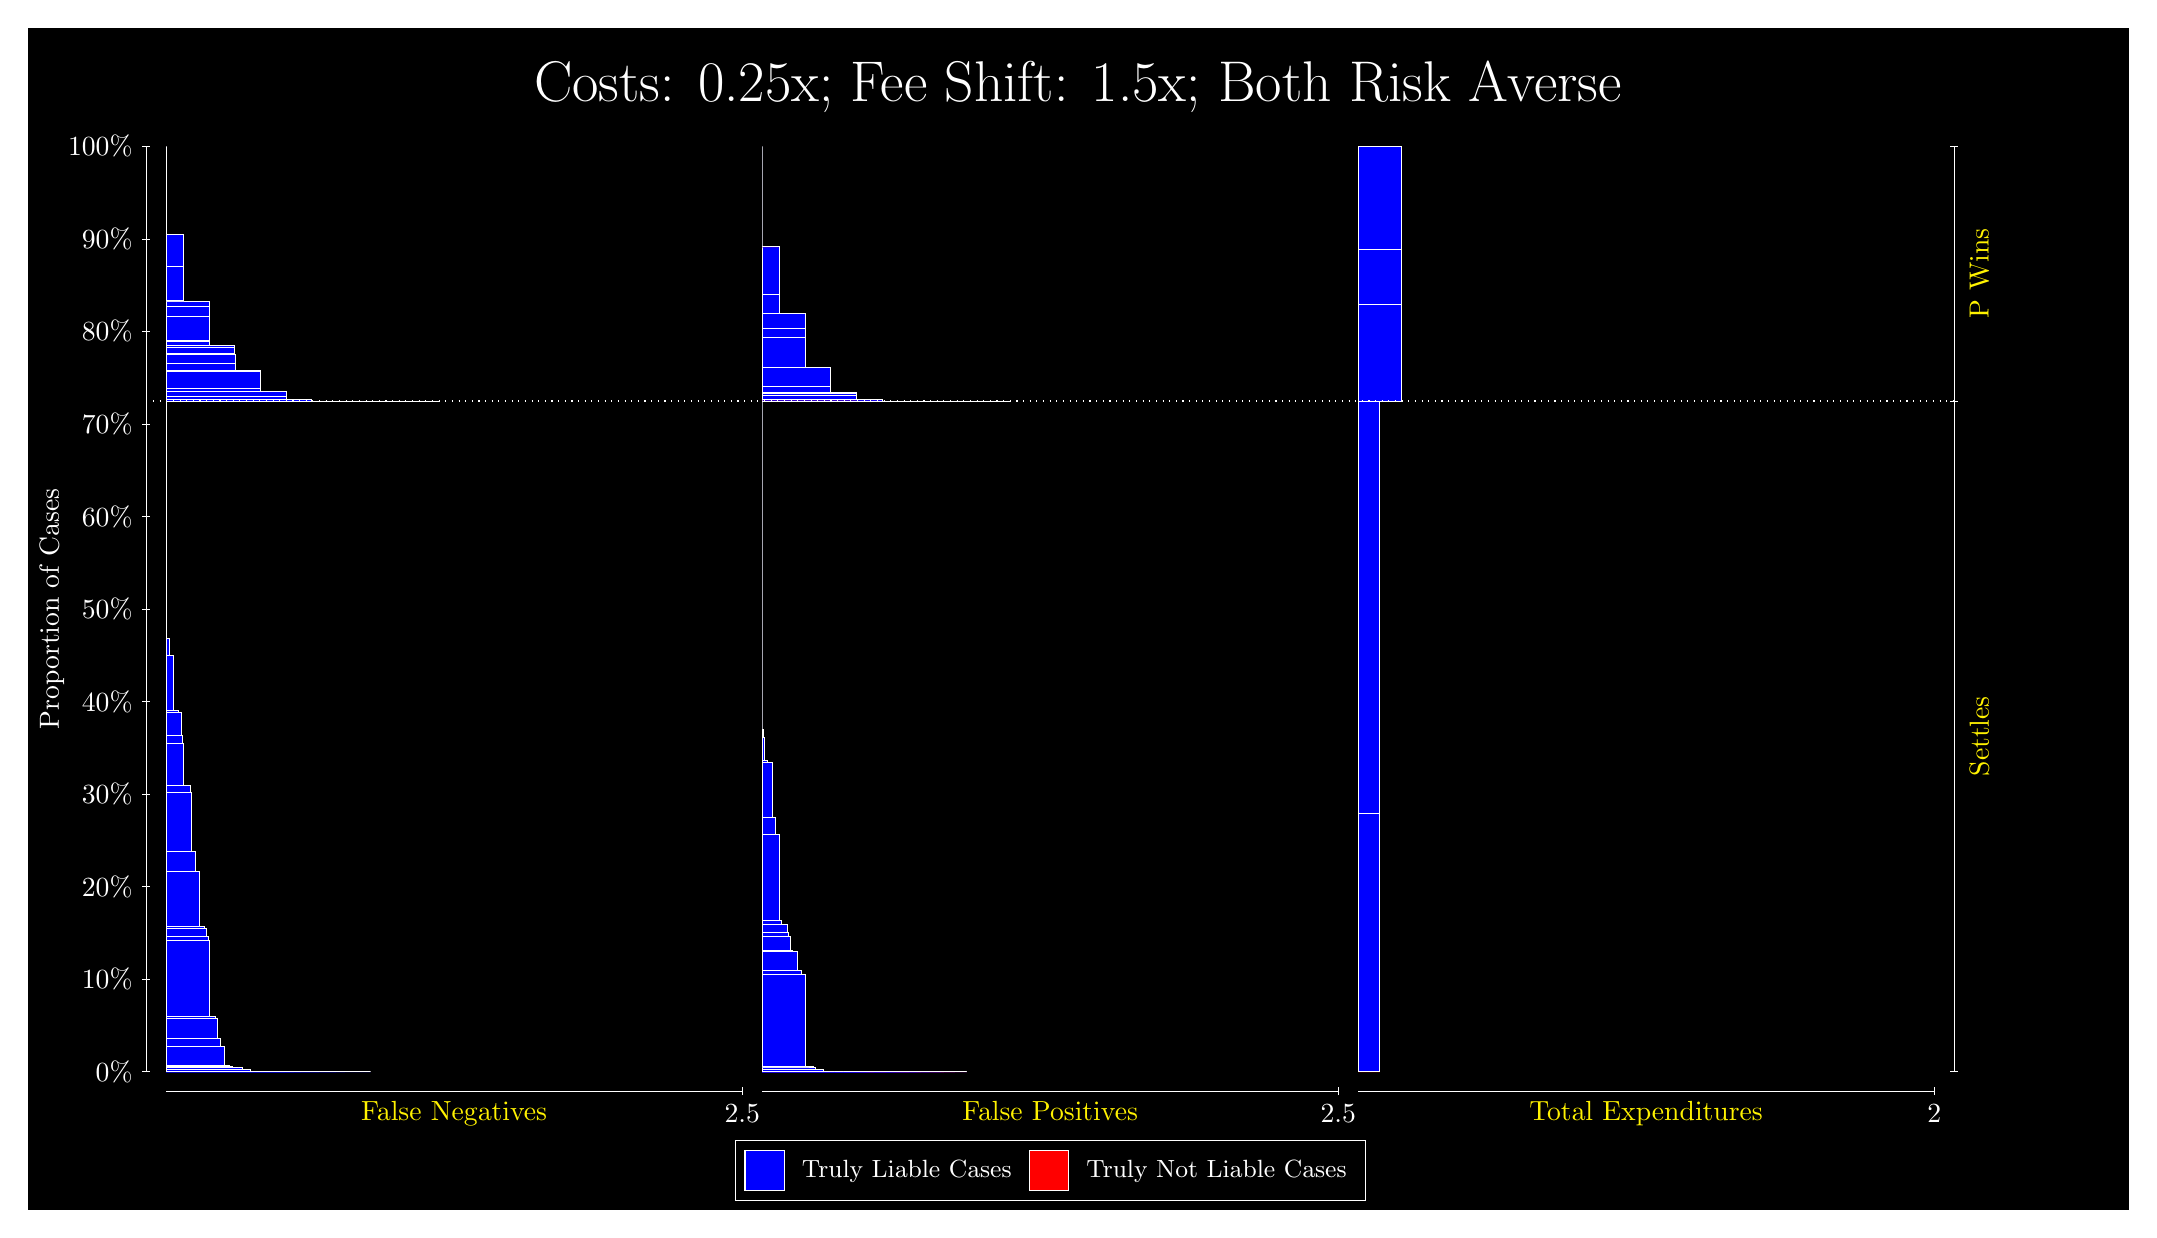
\begin{tikzpicture}
\draw[fill=black] (0,0) rectangle (26.667,15);
\draw[text=white] (0,13.5) rectangle (26.667,15) node[midway] {\huge Costs: 0.25x; Fee Shift: 1.5x; Both Risk Averse};
\draw[white, very thin] (1.5,1.75) -- (1.5,13.5);
\node[rotate=90, text=white, anchor=center] at (0.3, 7.625) {Proportion of Cases};
\draw[white, very thin] (1.45,1.75) -- (1.55,1.75);
\node[text=white, anchor=east] at (1.45, 1.75) {0\%};
\draw[white, very thin] (1.45,2.925) -- (1.55,2.925);
\node[text=white, anchor=east] at (1.45, 2.925) {10\%};
\draw[white, very thin] (1.45,4.1) -- (1.55,4.1);
\node[text=white, anchor=east] at (1.45, 4.1) {20\%};
\draw[white, very thin] (1.45,5.275) -- (1.55,5.275);
\node[text=white, anchor=east] at (1.45, 5.275) {30\%};
\draw[white, very thin] (1.45,6.45) -- (1.55,6.45);
\node[text=white, anchor=east] at (1.45, 6.45) {40\%};
\draw[white, very thin] (1.45,7.625) -- (1.55,7.625);
\node[text=white, anchor=east] at (1.45, 7.625) {50\%};
\draw[white, very thin] (1.45,8.8) -- (1.55,8.8);
\node[text=white, anchor=east] at (1.45, 8.8) {60\%};
\draw[white, very thin] (1.45,9.975) -- (1.55,9.975);
\node[text=white, anchor=east] at (1.45, 9.975) {70\%};
\draw[white, very thin] (1.45,11.15) -- (1.55,11.15);
\node[text=white, anchor=east] at (1.45, 11.15) {80\%};
\draw[white, very thin] (1.45,12.325) -- (1.55,12.325);
\node[text=white, anchor=east] at (1.45, 12.325) {90\%};
\draw[white, very thin] (1.45,13.5) -- (1.55,13.5);
\node[text=white, anchor=east] at (1.45, 13.5) {100\%};

\draw[white, very thin] (24.457,1.75) -- (24.457,13.5);
\draw[white, very thin] (24.407,1.75) -- (24.507,1.75);
\node[anchor=west] at (24.407, 1.75) {};
\draw[white, very thin] (24.407,10.265) -- (24.507,10.265);
\node[anchor=west] at (24.407, 10.265) {};
\draw[white, very thin] (24.407,13.5) -- (24.507,13.5);
\node[anchor=west] at (24.407, 13.5) {};

\draw[white, very thin, fill=blue] (1.75,1.75) rectangle (4.3482,1.75);
\draw[white, very thin, fill=blue] (1.75,1.75) rectangle (4.0229,1.75);
\draw[white, very thin, fill=blue] (1.75,1.75) rectangle (3.9091,1.75);
\draw[white, very thin, fill=blue] (1.75,1.75) rectangle (3.6976,1.75);
\draw[white, very thin, fill=blue] (1.75,1.75) rectangle (3.5838,1.75);
\draw[white, very thin, fill=blue] (1.75,1.75) rectangle (3.4699,1.75);
\draw[white, very thin, fill=blue] (1.75,1.75) rectangle (3.3723,1.75);
\draw[white, very thin, fill=blue] (1.75,1.75) rectangle (3.3236,1.75);
\draw[white, very thin, fill=blue] (1.75,1.75) rectangle (3.2585,1.75);
\draw[white, very thin, fill=blue] (1.75,1.75) rectangle (3.1447,1.7506);
\draw[white, very thin, fill=blue] (1.75,1.7506) rectangle (3.0471,1.7511);
\draw[white, very thin, fill=blue] (1.75,1.7511) rectangle (3.0308,1.7511);
\draw[white, very thin, fill=blue] (1.75,1.7511) rectangle (2.9983,1.7511);
\draw[white, very thin, fill=blue] (1.75,1.7511) rectangle (2.9332,1.7513);
\draw[white, very thin, fill=blue] (1.75,1.7513) rectangle (2.8844,1.7516);
\draw[white, very thin, fill=blue] (1.75,1.7516) rectangle (2.8194,1.7761);
\draw[white, very thin, fill=blue] (1.75,1.7761) rectangle (2.7218,1.8004);
\draw[white, very thin, fill=blue] (1.75,1.8004) rectangle (2.7055,1.8024);
\draw[white, very thin, fill=blue] (1.75,1.8024) rectangle (2.673,1.8024);
\draw[white, very thin, fill=blue] (1.75,1.8024) rectangle (2.6079,1.8087);
\draw[white, very thin, fill=blue] (1.75,1.8087) rectangle (2.5917,1.8186);
\draw[white, very thin, fill=blue] (1.75,1.8186) rectangle (2.5591,1.8238);
\draw[white, very thin, fill=blue] (1.75,1.8238) rectangle (2.4941,2.0723);
\draw[white, very thin, fill=blue] (1.75,2.0723) rectangle (2.4453,2.1745);
\draw[white, very thin, fill=blue] (1.75,2.1745) rectangle (2.3965,2.425);
\draw[white, very thin, fill=blue] (1.75,2.425) rectangle (2.3802,2.4554);
\draw[white, very thin, fill=blue] (1.75,2.4554) rectangle (2.3477,2.4554);
\draw[white, very thin, fill=blue] (1.75,2.4554) rectangle (2.2989,3.4144);
\draw[white, very thin, fill=blue] (1.75,3.4144) rectangle (2.2827,3.4682);
\draw[white, very thin, fill=blue] (1.75,3.4682) rectangle (2.2664,3.5668);
\draw[white, very thin, fill=blue] (1.75,3.5668) rectangle (2.2339,3.5908);
\draw[white, very thin, fill=blue] (1.75,3.5908) rectangle (2.1688,4.2888);
\draw[white, very thin, fill=blue] (1.75,4.2888) rectangle (2.12,4.5436);
\draw[white, very thin, fill=blue] (1.75,4.5436) rectangle (2.0712,5.2994);
\draw[white, very thin, fill=blue] (1.75,5.2994) rectangle (2.055,5.387);
\draw[white, very thin, fill=blue] (1.75,5.387) rectangle (2.0224,5.387);
\draw[white, very thin, fill=blue] (1.75,5.387) rectangle (1.9736,5.9135);
\draw[white, very thin, fill=blue] (1.75,5.9135) rectangle (1.9574,6.0252);
\draw[white, very thin, fill=blue] (1.75,6.0252) rectangle (1.9411,6.3098);
\draw[white, very thin, fill=blue] (1.75,6.3098) rectangle (1.9086,6.334);
\draw[white, very thin, fill=blue] (1.75,6.334) rectangle (1.8435,7.032);
\draw[white, very thin, fill=blue] (1.75,7.032) rectangle (1.7947,7.2567);
\draw[white, very thin, fill=red] (1.75,7.2567) rectangle (1.75,7.2567);
\draw[white, very thin, fill=blue] (1.75,7.2567) rectangle (1.75,10.265);
\draw[white, very thin, fill=blue] (1.75,10.265) rectangle (5.2265,10.265);
\draw[white, very thin, fill=blue] (1.75,10.265) rectangle (4.9012,10.265);
\draw[white, very thin, fill=blue] (1.75,10.265) rectangle (4.5759,10.265);
\draw[white, very thin, fill=blue] (1.75,10.265) rectangle (4.5759,10.265);
\draw[white, very thin, fill=blue] (1.75,10.265) rectangle (4.2506,10.265);
\draw[white, very thin, fill=blue] (1.75,10.265) rectangle (4.2506,10.265);
\draw[white, very thin, fill=blue] (1.75,10.265) rectangle (4.2465,10.265);
\draw[white, very thin, fill=blue] (1.75,10.265) rectangle (3.9253,10.268);
\draw[white, very thin, fill=blue] (1.75,10.268) rectangle (3.9213,10.268);
\draw[white, very thin, fill=blue] (1.75,10.268) rectangle (3.6,10.288);
\draw[white, very thin, fill=blue] (1.75,10.288) rectangle (3.596,10.288);
\draw[white, very thin, fill=blue] (1.75,10.288) rectangle (3.2748,10.324);
\draw[white, very thin, fill=blue] (1.75,10.324) rectangle (3.2748,10.392);
\draw[white, very thin, fill=blue] (1.75,10.392) rectangle (3.2707,10.392);
\draw[white, very thin, fill=blue] (1.75,10.392) rectangle (3.2707,10.392);
\draw[white, very thin, fill=blue] (1.75,10.392) rectangle (2.9495,10.427);
\draw[white, very thin, fill=blue] (1.75,10.427) rectangle (2.9495,10.643);
\draw[white, very thin, fill=blue] (1.75,10.643) rectangle (2.9454,10.646);
\draw[white, very thin, fill=blue] (1.75,10.646) rectangle (2.9454,10.647);
\draw[white, very thin, fill=blue] (1.75,10.647) rectangle (2.9454,10.651);
\draw[white, very thin, fill=blue] (1.75,10.651) rectangle (2.6242,10.748);
\draw[white, very thin, fill=blue] (1.75,10.748) rectangle (2.6242,10.856);
\draw[white, very thin, fill=blue] (1.75,10.856) rectangle (2.6242,10.86);
\draw[white, very thin, fill=blue] (1.75,10.86) rectangle (2.6201,10.869);
\draw[white, very thin, fill=blue] (1.75,10.869) rectangle (2.6201,10.947);
\draw[white, very thin, fill=blue] (1.75,10.947) rectangle (2.6201,10.976);
\draw[white, very thin, fill=blue] (1.75,10.976) rectangle (2.2989,11.026);
\draw[white, very thin, fill=blue] (1.75,11.026) rectangle (2.2948,11.042);
\draw[white, very thin, fill=blue] (1.75,11.042) rectangle (2.2948,11.343);
\draw[white, very thin, fill=blue] (1.75,11.343) rectangle (2.2948,11.463);
\draw[white, very thin, fill=blue] (1.75,11.463) rectangle (2.2948,11.535);
\draw[white, very thin, fill=blue] (1.75,11.535) rectangle (1.9736,11.535);
\draw[white, very thin, fill=blue] (1.75,11.535) rectangle (1.9736,11.539);
\draw[white, very thin, fill=blue] (1.75,11.539) rectangle (1.9736,11.539);
\draw[white, very thin, fill=blue] (1.75,11.539) rectangle (1.9696,11.972);
\draw[white, very thin, fill=blue] (1.75,11.972) rectangle (1.9696,12.384);
\draw[white, very thin, fill=red] (1.75,12.384) rectangle (1.75,12.384);
\draw[white, very thin, fill=blue] (1.75,12.384) rectangle (1.75,13.5);
\draw[white, very thin, fill=red] (9.3189,1.75) rectangle (11.917,1.75);
\draw[white, very thin, fill=blue] (9.3189,1.75) rectangle (11.917,1.75);
\draw[white, very thin, fill=red] (9.3189,1.75) rectangle (11.771,1.75);
\draw[white, very thin, fill=blue] (9.3189,1.75) rectangle (11.771,1.75);
\draw[white, very thin, fill=red] (9.3189,1.75) rectangle (11.624,1.75);
\draw[white, very thin, fill=blue] (9.3189,1.75) rectangle (11.624,1.75);
\draw[white, very thin, fill=blue] (9.3189,1.75) rectangle (11.592,1.75);
\draw[white, very thin, fill=blue] (9.3189,1.75) rectangle (11.445,1.75);
\draw[white, very thin, fill=red] (9.3189,1.75) rectangle (11.332,1.75);
\draw[white, very thin, fill=blue] (9.3189,1.75) rectangle (11.332,1.75);
\draw[white, very thin, fill=blue] (9.3189,1.75) rectangle (11.299,1.75);
\draw[white, very thin, fill=blue] (9.3189,1.75) rectangle (11.266,1.75);
\draw[white, very thin, fill=red] (9.3189,1.75) rectangle (11.185,1.75);
\draw[white, very thin, fill=blue] (9.3189,1.75) rectangle (11.185,1.75);
\draw[white, very thin, fill=blue] (9.3189,1.75) rectangle (11.12,1.75);
\draw[white, very thin, fill=blue] (9.3189,1.75) rectangle (11.006,1.75);
\draw[white, very thin, fill=blue] (9.3189,1.75) rectangle (10.974,1.75);
\draw[white, very thin, fill=blue] (9.3189,1.75) rectangle (10.941,1.75);
\draw[white, very thin, fill=red] (9.3189,1.75) rectangle (10.892,1.75);
\draw[white, very thin, fill=blue] (9.3189,1.75) rectangle (10.892,1.75);
\draw[white, very thin, fill=blue] (9.3189,1.75) rectangle (10.86,1.75);
\draw[white, very thin, fill=blue] (9.3189,1.75) rectangle (10.795,1.75);
\draw[white, very thin, fill=red] (9.3189,1.75) rectangle (10.746,1.75);
\draw[white, very thin, fill=blue] (9.3189,1.75) rectangle (10.746,1.75);
\draw[white, very thin, fill=blue] (9.3189,1.75) rectangle (10.681,1.75);
\draw[white, very thin, fill=blue] (9.3189,1.75) rectangle (10.648,1.75);
\draw[white, very thin, fill=blue] (9.3189,1.75) rectangle (10.616,1.75);
\draw[white, very thin, fill=blue] (9.3189,1.75) rectangle (10.567,1.75);
\draw[white, very thin, fill=blue] (9.3189,1.75) rectangle (10.535,1.75);
\draw[white, very thin, fill=blue] (9.3189,1.75) rectangle (10.47,1.75);
\draw[white, very thin, fill=blue] (9.3189,1.75) rectangle (10.421,1.7506);
\draw[white, very thin, fill=blue] (9.3189,1.7506) rectangle (10.356,1.7506);
\draw[white, very thin, fill=blue] (9.3189,1.7506) rectangle (10.323,1.7511);
\draw[white, very thin, fill=red] (9.3189,1.7511) rectangle (10.307,1.7511);
\draw[white, very thin, fill=blue] (9.3189,1.7511) rectangle (10.307,1.7514);
\draw[white, very thin, fill=blue] (9.3189,1.7514) rectangle (10.291,1.7515);
\draw[white, very thin, fill=blue] (9.3189,1.7515) rectangle (10.242,1.7515);
\draw[white, very thin, fill=blue] (9.3189,1.7515) rectangle (10.209,1.7517);
\draw[white, very thin, fill=blue] (9.3189,1.7517) rectangle (10.144,1.7539);
\draw[white, very thin, fill=blue] (9.3189,1.7539) rectangle (10.095,1.7784);
\draw[white, very thin, fill=blue] (9.3189,1.7784) rectangle (10.03,1.7786);
\draw[white, very thin, fill=blue] (9.3189,1.7786) rectangle (9.9979,1.8002);
\draw[white, very thin, fill=blue] (9.3189,1.8002) rectangle (9.9816,1.8074);
\draw[white, very thin, fill=blue] (9.3189,1.8074) rectangle (9.9654,1.8126);
\draw[white, very thin, fill=blue] (9.3189,1.8126) rectangle (9.9166,1.8126);
\draw[white, very thin, fill=blue] (9.3189,1.8126) rectangle (9.884,1.8187);
\draw[white, very thin, fill=red] (9.3189,1.8187) rectangle (9.8678,1.8187);
\draw[white, very thin, fill=blue] (9.3189,1.8187) rectangle (9.8678,2.9828);
\draw[white, very thin, fill=blue] (9.3189,2.9828) rectangle (9.819,3.0316);
\draw[white, very thin, fill=blue] (9.3189,3.0316) rectangle (9.7702,3.2801);
\draw[white, very thin, fill=blue] (9.3189,3.2801) rectangle (9.7051,3.2851);
\draw[white, very thin, fill=blue] (9.3189,3.2851) rectangle (9.6726,3.4626);
\draw[white, very thin, fill=blue] (9.3189,3.4626) rectangle (9.6563,3.517);
\draw[white, very thin, fill=blue] (9.3189,3.517) rectangle (9.6401,3.6258);
\draw[white, very thin, fill=blue] (9.3189,3.6258) rectangle (9.5913,3.6258);
\draw[white, very thin, fill=blue] (9.3189,3.6258) rectangle (9.5588,3.6746);
\draw[white, very thin, fill=blue] (9.3189,3.6746) rectangle (9.5425,4.7582);
\draw[white, very thin, fill=blue] (9.3189,4.7582) rectangle (9.4937,4.9829);
\draw[white, very thin, fill=blue] (9.3189,4.9829) rectangle (9.4449,5.681);
\draw[white, very thin, fill=blue] (9.3189,5.681) rectangle (9.3799,5.7051);
\draw[white, very thin, fill=blue] (9.3189,5.7051) rectangle (9.3473,5.9897);
\draw[white, very thin, fill=blue] (9.3189,5.9897) rectangle (9.3311,6.1014);
\draw[white, very thin, fill=blue] (9.3189,6.1014) rectangle (9.3189,10.265);
\draw[white, very thin, fill=red] (9.3189,10.265) rectangle (12.466,10.265);
\draw[white, very thin, fill=blue] (9.3189,10.265) rectangle (12.466,10.265);
\draw[white, very thin, fill=red] (9.3189,10.265) rectangle (12.141,10.265);
\draw[white, very thin, fill=blue] (9.3189,10.265) rectangle (12.141,10.265);
\draw[white, very thin, fill=red] (9.3189,10.265) rectangle (11.815,10.265);
\draw[white, very thin, fill=blue] (9.3189,10.265) rectangle (11.815,10.265);
\draw[white, very thin, fill=blue] (9.3189,10.265) rectangle (11.815,10.265);
\draw[white, very thin, fill=blue] (9.3189,10.265) rectangle (11.49,10.265);
\draw[white, very thin, fill=red] (9.3189,10.265) rectangle (11.49,10.265);
\draw[white, very thin, fill=blue] (9.3189,10.265) rectangle (11.49,10.265);
\draw[white, very thin, fill=red] (9.3189,10.265) rectangle (11.165,10.265);
\draw[white, very thin, fill=blue] (9.3189,10.265) rectangle (11.165,10.267);
\draw[white, very thin, fill=red] (9.3189,10.267) rectangle (11.161,10.267);
\draw[white, very thin, fill=blue] (9.3189,10.267) rectangle (11.161,10.267);
\draw[white, very thin, fill=red] (9.3189,10.267) rectangle (10.84,10.267);
\draw[white, very thin, fill=blue] (9.3189,10.267) rectangle (10.84,10.282);
\draw[white, very thin, fill=red] (9.3189,10.282) rectangle (10.835,10.282);
\draw[white, very thin, fill=blue] (9.3189,10.282) rectangle (10.835,10.282);
\draw[white, very thin, fill=blue] (9.3189,10.282) rectangle (10.835,10.282);
\draw[white, very thin, fill=red] (9.3189,10.282) rectangle (10.514,10.282);
\draw[white, very thin, fill=blue] (9.3189,10.282) rectangle (10.514,10.334);
\draw[white, very thin, fill=blue] (9.3189,10.334) rectangle (10.514,10.359);
\draw[white, very thin, fill=blue] (9.3189,10.359) rectangle (10.514,10.374);
\draw[white, very thin, fill=blue] (9.3189,10.374) rectangle (10.51,10.374);
\draw[white, very thin, fill=red] (9.3189,10.374) rectangle (10.51,10.374);
\draw[white, very thin, fill=blue] (9.3189,10.374) rectangle (10.51,10.374);
\draw[white, very thin, fill=red] (9.3189,10.374) rectangle (10.189,10.374);
\draw[white, very thin, fill=blue] (9.3189,10.374) rectangle (10.189,10.45);
\draw[white, very thin, fill=blue] (9.3189,10.45) rectangle (10.189,10.698);
\draw[white, very thin, fill=blue] (9.3189,10.698) rectangle (10.185,10.698);
\draw[white, very thin, fill=red] (9.3189,10.698) rectangle (10.185,10.698);
\draw[white, very thin, fill=blue] (9.3189,10.698) rectangle (10.185,10.698);
\draw[white, very thin, fill=blue] (9.3189,10.698) rectangle (9.8637,11.073);
\draw[white, very thin, fill=blue] (9.3189,11.073) rectangle (9.8637,11.193);
\draw[white, very thin, fill=blue] (9.3189,11.193) rectangle (9.8637,11.381);
\draw[white, very thin, fill=blue] (9.3189,11.381) rectangle (9.8597,11.381);
\draw[white, very thin, fill=red] (9.3189,11.381) rectangle (9.8597,11.381);
\draw[white, very thin, fill=blue] (9.3189,11.381) rectangle (9.8597,11.381);
\draw[white, very thin, fill=blue] (9.3189,11.381) rectangle (9.5384,11.623);
\draw[white, very thin, fill=blue] (9.3189,11.623) rectangle (9.5384,12.226);
\draw[white, very thin, fill=blue] (9.3189,12.226) rectangle (9.5344,12.226);
\draw[white, very thin, fill=blue] (9.3189,12.226) rectangle (9.5344,12.226);
\draw[white, very thin, fill=red] (9.3189,12.226) rectangle (9.5344,12.226);
\draw[white, very thin, fill=blue] (9.3189,12.226) rectangle (9.5344,12.23);
\draw[white, very thin, fill=blue] (9.3189,12.23) rectangle (9.5344,12.23);
\draw[white, very thin, fill=red] (9.3189,12.23) rectangle (9.3189,12.23);
\draw[white, very thin, fill=blue] (9.3189,12.23) rectangle (9.3189,13.5);
\draw[white, very thin, fill=red] (16.888,1.75) rectangle (17.162,1.75);
\draw[white, very thin, fill=blue] (16.888,1.75) rectangle (17.162,5.0286);
\draw[white, very thin, fill=red] (16.888,5.0286) rectangle (17.162,5.0286);
\draw[white, very thin, fill=blue] (16.888,5.0286) rectangle (17.162,10.265);
\draw[white, very thin, fill=red] (16.888,10.265) rectangle (17.437,10.265);
\draw[white, very thin, fill=blue] (16.888,10.265) rectangle (17.437,11.498);
\draw[white, very thin, fill=red] (16.888,11.498) rectangle (17.437,11.498);
\draw[white, very thin, fill=blue] (16.888,11.498) rectangle (17.437,12.193);
\draw[white, very thin, fill=red] (16.888,12.193) rectangle (17.437,12.193);
\draw[white, very thin, fill=blue] (16.888,12.193) rectangle (17.437,13.5);
\draw[white, dotted] (1.5,10.265) -- (24.457,10.265);
\draw[white, very thin] (1.75,1.5) -- (9.0689,1.5);
\node[text=yellow, anchor=north] at (5.4094, 1.5) {False Negatives};
\draw[white, very thin] (9.0689,1.45) -- (9.0689,1.55);
\node[text=white, anchor=north] at (9.0689, 1.45) {2.5};

\draw[white, very thin] (9.3189,1.5) -- (16.638,1.5);
\node[text=yellow, anchor=north] at (12.978, 1.5) {False Positives};
\draw[white, very thin] (16.638,1.45) -- (16.638,1.55);
\node[text=white, anchor=north] at (16.638, 1.45) {2.5};

\draw[white, very thin] (16.888,1.5) -- (24.207,1.5);
\node[text=yellow, anchor=north] at (20.547, 1.5) {Total Expenditures};
\draw[white, very thin] (24.207,1.45) -- (24.207,1.55);
\node[text=white, anchor=north] at (24.207, 1.45) {2};

\node[text=yellow, centered, rotate=90] at (24.777, 6.0075) {Settles};
\node[text=yellow, centered, rotate=90] at (24.777, 11.882) {P Wins};

\draw (12.978300999999998,1.5) node[draw=none] (baseCoordinate) {};
\begin{scope}[align=center]
        \matrix[scale=0.5, draw=white, below=0.5cm of baseCoordinate, nodes={draw}, column sep=0.1cm]{
            \node[rectangle, draw, minimum width=0.5cm, minimum height=0.5cm, fill=blue] {}; &
            \node[draw=none, font=\small, text=white] (B) {Truly Liable Cases}; &
            \node[rectangle, draw, minimum width=0.5cm, minimum height=0.5cm, fill=red] {}; &
            \node[draw=none, font=\small, text=white] (B) {Truly Not Liable Cases}; \\
            };
\end{scope}

\end{tikzpicture}
\end{document}